\documentclass[11pt]{article}
\usepackage[T1]{fontenc}
\usepackage[utf8]{inputenc}
\usepackage{natbib,graphicx,amsmath,amssymb,booktabs,longtable,titlesec,caption,xcolor}
\usepackage[a4paper,margin=2cm]{geometry}
\usepackage[hidelinks]{hyperref}
\bibliographystyle{apalike}
\setlength{\parskip}{0.5em}
\setlength{\parindent}{0pt}
\titleformat{\section}{\normalfont\Large\bfseries}{\thesection}{1em}{}
\titleformat{\subsection}{\normalfont\large\bfseries}{\thesubsection}{1em}{}
\titleformat{\subsubsection}{\normalfont\normalsize\bfseries}{\thesubsubsection}{1em}{}
\captionsetup{font=footnotesize,labelfont=bf}
\newcommand{\wg}{w_{\mathrm g}}
\newcommand{\wmax}{w_{\max}}

\begin{document}
\hypersetup{pageanchor=false}
\begin{titlepage}
\centering\vspace*{3cm}
{\Huge\bfseries Separating Sample and Medium in Brillouin Microscopy\par}
\vspace{2cm}{\Large Noah Klugman\par}
\vspace{0.3cm}{\large Student ID: 24948806\par}
\vfill{\large 32931 Technology Research Preparation\par}
\vspace{0.3cm}{\large University of Technology Sydney\par}
\vspace{1cm}{\large \today\par}
\end{titlepage}
\hypersetup{pageanchor=true}

\section*{List of Symbols}
Frequency variables are ordinary frequencies, expressed in GHz in the simulations; they are not angular frequencies. Indices $i$, $k$ and $m$ denote scan positions, spectral components and frequency bins. Hats denote estimates.
\small
\begin{longtable}{@{}p{0.25\textwidth}p{0.69\textwidth}@{}}
\toprule Symbol & Meaning \\ \midrule\endfirsthead
\toprule Symbol & Meaning \\ \midrule\endhead
$f$, $f_{\mathrm B}$ & Frequency shift coordinate and positive Brillouin frequency shift (BFS). \\
$\Gamma$, $\Gamma_h$ & Intrinsic Brillouin FWHM and instrument-response FWHM. \\
$A$, $A_0$ & Integrated local spectral response and its water reference value. \\
$n$, $v_{\mathrm L}$, $\lambda_0$, $\theta$ & Refractive index, longitudinal acoustic phase velocity, vacuum laser wavelength and scattering angle. \\
$\rho$, $M'$, $M''$, $E$ & Density, longitudinal storage and loss moduli, and Young's modulus. \\
$\wg$, $\wmax$ & Glycerol mass fraction and maximum prescribed mass fraction. \\
$a$, $b$, $\delta_A$ & Coefficients controlling BFS, linewidth and integrated intensity. \\
$\mathbf r$, $r_s$, $d$, $\beta$ & Spatial coordinate, sample radius, normalised radius and concentration-profile exponent. \\
$W_i(z)$, $L_z$ & Normalised axial collection weighting and collection length. \\
$R(f;\wg)$, $s_i(f)$ & Local spectral response and depth-averaged ideal spectrum. \\
$h$, $*$, $b_i(f)$ & Unit-area instrument line-spread function, convolution and additive spectral background. \\
$a_{ik}$, $p_{ik}$ & Collection-weighted component coefficient and normalised coefficient. \\
$\mathbf Y$, $\mathbf C$, $\mathbf S$, $\mathbf D$ & Dataset matrix, coefficients, component spectra and reference dictionary. \\
$\mu_{im}$, $N_{im}$ & Expected and sampled photon counts. \\
$t_i$, $\kappa$, $P$ & Acquisition time, conversion to photon rate and reference photon budget. \\
$\nu_i$, $\pi_{ij}$ & Collection-weighted concentration probability measure and discretised bin mass. \\
$\eta$, $\mathbf L$ & Regularisation strength and second-difference matrix. \\
$G(f_{\mathrm B})$, $H(f_{\mathrm B})$ & Unknown linewidth and integrated-intensity relationships. \\
$F_i$, $\widehat F_i$, $W_{1,i}$ & True and recovered cumulative distributions and Wasserstein distance. \\
MAE, NRMSE & Mean absolute error and relative spectral root mean square error. \\
\bottomrule
\end{longtable}
\normalsize\clearpage\tableofcontents\clearpage

\section{Introduction}
\label{sec:introduction}
\subsection{Biomechanics and biological function}

Measuring the mechanical properties of biological samples is difficult because different techniques probe different responses, length scales and timescales. A mechanical measurement therefore needs to be interpreted in terms of how it was obtained, rather than treated as a universal measure of stiffness. This matters when using mechanics to distinguish cells or understand how their surroundings influence their behaviour. Two cells can have similar appearances while responding differently to an applied force, as illustrated schematically in Figure~\ref{fig:healthy-cancer}.

Mechanical properties can reveal differences associated with disease and can also influence biological function. \citet{cross2007} used atomic force microscopy (AFM) to examine cells collected from the pleural fluids of patients with suspected cancer. Metastatic cancer cells were softer than benign cells in the same samples despite similarities in their appearance. This result concerns the cell populations and measurement conditions studied; it does not establish that every cancer cell is softer than every healthy cell. In a different setting, \citet{engler2006} showed that matrix elasticity influenced the lineage specification of mesenchymal stem cells. Together, these examples motivate mechanical measurements as a source of information that complements microscopy images.

\begin{figure}[htbp]\centering
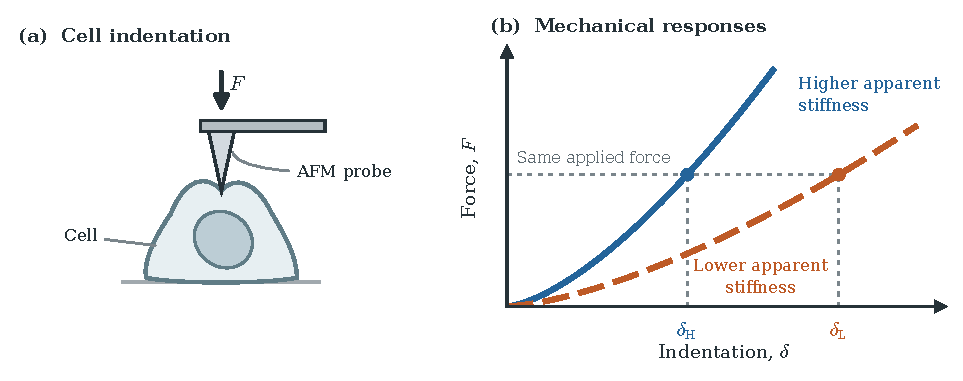
\includegraphics[width=.72\linewidth]{figures/figure_01_cell_mechanics.pdf}
\caption{Similar appearances can conceal different mechanical responses. An AFM probe applies force to a cell; at the same force, the higher-stiffness illustrative response has less indentation. The curves are schematic.}
\label{fig:healthy-cancer}\end{figure}

AFM measures local mechanical response by indenting a sample with a cantilever tip and relating the applied force to the resulting deformation. It can perform indentation at nanometre or micrometre scales depending on the probe and experiment; AFM indentation and nanoindentation should therefore not be presented as entirely separate physical principles. The inferred properties depend on the loading conditions and mechanical model. Brillouin microscopy provides a complementary optical measurement of the response to acoustic waves at GHz frequencies, rather than reproducing the same response measured in a slow indentation experiment \citep{prevedel2019}.

\subsection{Brillouin scattering and mechanical interpretation}
\label{sec:brillouin}

Brillouin microscopy measures small frequency changes in scattered light caused by its interaction with acoustic excitations. In \emph{spontaneous Brillouin scattering}, thermally excited acoustic phonons exchange energy with the incident light: phonon creation produces the lower-frequency Stokes peak, while phonon annihilation produces the higher-frequency anti-Stokes peak. A spectrum is acquired at each scan position, so a two-dimensional scan contains a frequency axis in addition to its two spatial axes. Figure~\ref{fig:brillouin_setup} illustrates this acquisition process, and Figure~\ref{fig:brillouin_spectrum} identifies the spectral features used in the analysis \citep{prevedel2019}.

\begin{figure}[htbp]\centering
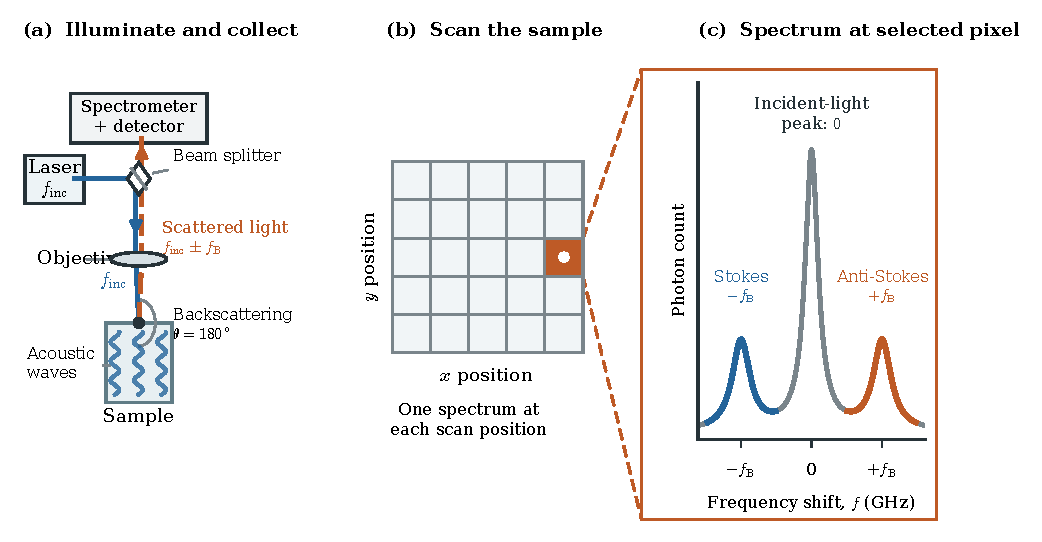
\includegraphics[width=1.0\linewidth]{figures/figure_02_brillouin_scan.pdf}
\caption{How Brillouin microscopy produces a spectral image. (a) Incident light is focused into a sample and backscattered light is directed to a separate spectrometer and detector. Acoustic-wave motifs are symbolic. (b) Each spatial scan position contains a spectrum. (c) Expanding guides connect one pixel to its cartoon photon-count spectrum. The peaks, geometry and counts are schematic; the angle is ideal backscattering.}
\label{fig:brillouin_setup}\end{figure}

For a homogeneous material, the magnitude of the Brillouin frequency shift is
\begin{equation}
 f_{\mathrm B}=\frac{2nv_{\mathrm L}}{\lambda_0}\sin\left(\frac{\theta}{2}\right).
 \label{eq:intro_brillouin_shift}
\end{equation}
Here $n$ is refractive index, $v_{\mathrm L}$ is longitudinal acoustic phase velocity, $\lambda_0$ is incident wavelength in vacuum and $\theta$ is the angle between incident and scattered optical wavevectors. Backscattering has $\theta=180^\circ$, giving $f_{\mathrm B}=2nv_{\mathrm L}/\lambda_0$. Throughout this thesis, $f_{\mathrm B}$ is an ordinary frequency rather than an angular frequency. The linewidth $\Gamma$ is the full width at half maximum (FWHM), also in ordinary frequency units.

The GHz longitudinal response differs from the unconfined response described by Young's modulus. For an isotropic material, the longitudinal storage modulus satisfies $M'=K'+4G'/3$, where $K'$ and $G'$ are bulk and shear storage moduli. In the weak-damping approximation,
\begin{equation}
 M'\simeq\rho v_{\mathrm L}^{\,2}
 =\rho\left[\frac{\lambda_0 f_{\mathrm B}}{2n\sin(\theta/2)}\right]^2,
 \qquad \frac{M''}{M'}\simeq\frac{\Gamma}{f_{\mathrm B}}.
 \label{eq:mechanical_moduli}
\end{equation}
These expressions require consistent units and an intrinsic linewidth corrected for instrumental effects. Longitudinal deformation involves compression with constrained transverse strain, whereas a uniaxial Young's-modulus measurement permits lateral deformation. Hydrated soft materials can consequently have a GHz longitudinal modulus on the GPa scale while their low-frequency Young's modulus is on the kPa scale; the two are not interchangeable measures \citep{bouvet2025}.

Hydration and composition further complicate the interpretation of Brillouin measurements. \citet{wu2018} demonstrated a strong influence of water content in hydrated materials, so a change in BFS should not automatically be labelled a change in low-frequency stiffness. This study will instead recover spectral parameters and spectral contributions. Converting those estimates into mechanical moduli would require additional material information and is outside its scope.

\begin{figure}[htbp]\centering
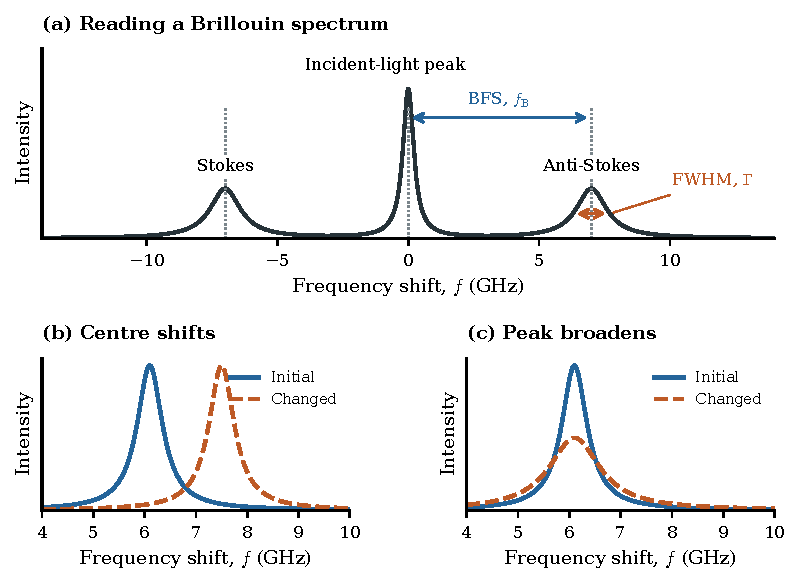
\includegraphics[width=1.0\linewidth]{figures/figure_03_spectral_features.pdf}
\caption{Reading a Brillouin spectrum. (a) BFS is the separation from the incident-light frequency, and FWHM is the width at half peak height. The lower panels distinguish (b) a centre shift from (c) increased linewidth. Curves are schematic; the simulation models only the positive-shift Brillouin band.}
\label{fig:brillouin_spectrum}\end{figure}

Different materials can produce distinct spectral responses. Figure~\ref{fig:water_plexiglas} introduces this contrast before the collection of mixed signals is considered.

\begin{figure}[htbp]\centering
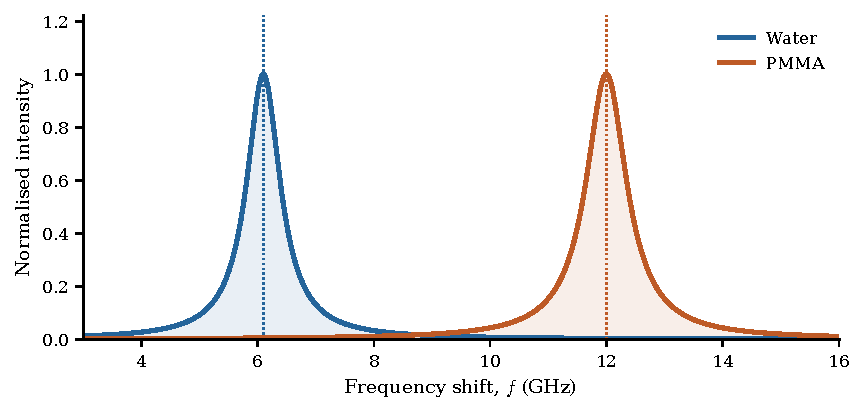
\includegraphics[width=1.0\linewidth]{figures/figure_04_material_responses.pdf}
\caption{Different materials can have separated Brillouin responses. These schematic water and Plexiglass peaks introduce material contrast; they are not the water--glycerol simulation calibration.}
\label{fig:water_plexiglas}\end{figure}

\subsection{Mixed spectra and measurement limitations}

A spectrum acquired at one scan position can contain contributions from several regions of the sample. The collection volume has a finite extent, and an elongated axial response can combine light from the sample and its surrounding medium. Figure~\ref{fig:collection_volume} illustrates this mixing. A change between neighbouring spectra may therefore reflect a changing mixture of fixed material responses, rather than a change in either material's local properties. The collection geometry is specified in Section~\ref{sec:geometry}; no experimental data are acquired in the present study.

\begin{figure}[htbp]\centering
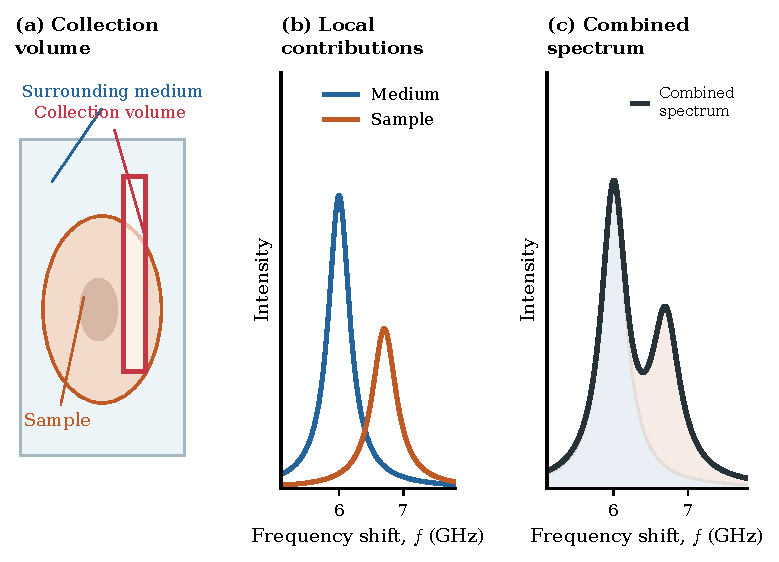
\includegraphics[width=1.0\linewidth]{figures/figure_05_collection_volume.pdf}
\caption{A finite collection volume can include sample and surrounding medium. Their weighted local responses combine into one measured spectrum. The colours identify contributions, not separate reconstructed depth positions.}
\label{fig:collection_volume}\end{figure}

Spectral overlap makes these contributions harder to distinguish. Well-separated material peaks, illustrated in Figure~\ref{fig:water_plexiglas}, can produce recognisable features, whereas nearby peaks can combine into a single broad or asymmetric response. Instrumental effects introduce a further change in shape: the recorded spectrum is the convolution of the incoming spectrum with the instrument line-spread function. Characterising that response permits correction through an instrument-aware fit or regularised deconvolution, although noise limits how well such a correction can recover intrinsic linewidths \citep{bouvet2025}. Figure~\ref{fig:single_peak_fit} illustrates why a plausible single-peak fit can still misrepresent a mixture.



Noise and drift affect a measurement in different ways and will be distinguished explicitly. Photon shot noise arises from counting statistics; detector read noise comes from the detection electronics; and background light adds photons that can also fluctuate. Drift changes the instrument's frequency or intensity response over time rather than merely adding independent random errors. Longer collection can reduce relative shot noise while increasing scan duration. Figure~\ref{fig:noise} illustrates how reducing exposure time at fixed photon rate increases relative shot noise in an otherwise unchanged mixed response. Its connected count traces use raw counts rather than area-normalised intensities. The primary simulations will isolate photon shot noise, with instrumental broadening treated separately as a deterministic response. This controlled choice does not imply that other effects are absent from a physical microscope.

\begin{figure}[htbp]\centering
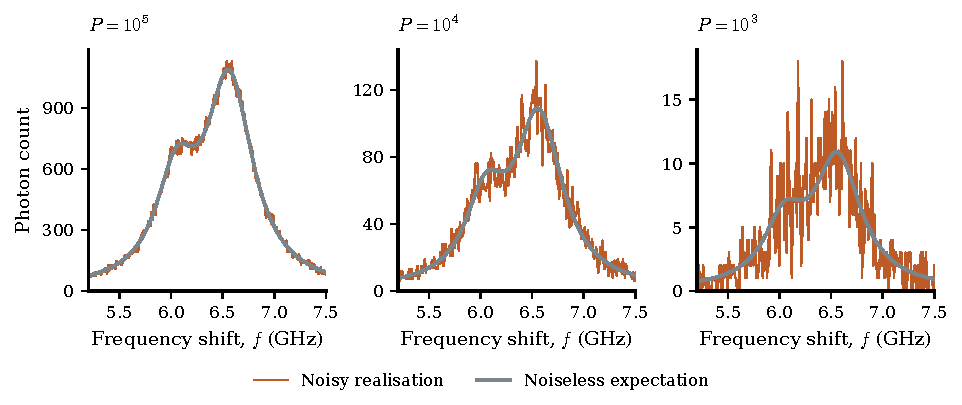
\includegraphics[width=1.0\linewidth]{figures/figure_06_exposure_noise.pdf}
\caption{Shorter exposure increases relative photon shot noise. Connected orange lines show independent Poisson-count realisations, with faint blue expected traces. The underlying mixed response and photon rate are fixed; only exposure changes. Raw-count axes change scale between panels. The illustrative scale is 1000 expected water-reference photons per second in the displayed 5.25--7.35 GHz band; these times are not an experimental calibration.}
\label{fig:noise}\end{figure}

\subsection{Recovering spectral contributions}

\emph{Spectral unmixing} estimates the responses contributing to a measured mixture and their weights. For a fixed set of component spectra, an additive model is
\begin{equation}
 y_i(f)=\sum_{k=1}^{K}a_{ik}R_k(f)+b_i(f)+\varepsilon_i(f),\qquad a_{ik}\geq0.
 \label{eq:linear_mixture}
\end{equation}
Here $R_k$ denotes a component response in the measurement domain, $a_{ik}$ is its coefficient, $b_i$ is an additive optical or detector background and $\varepsilon_i$ is the random measurement residual. The surrounding water is a material component, not the additive background. Instrumental broadening is incorporated into $R_k$ when fitting measured data. Coefficients depend on spectral normalisation and collection weighting, so they cannot automatically be interpreted as glycerol mass fractions.

A single-component fit provides an apparent peak position, linewidth and intensity, but does not explicitly separate the terms in Equation~\ref{eq:linear_mixture}. Its fitted peak can lie between the true component centres, and its width can reflect both intrinsic linewidth and component separation. Figure~\ref{fig:single_peak_fit} illustrates this distinction. The single-Lorentzian fit will therefore serve as a descriptive baseline, with its reconstruction error reported separately from any claim of component recovery.

\begin{figure}[htbp]\centering
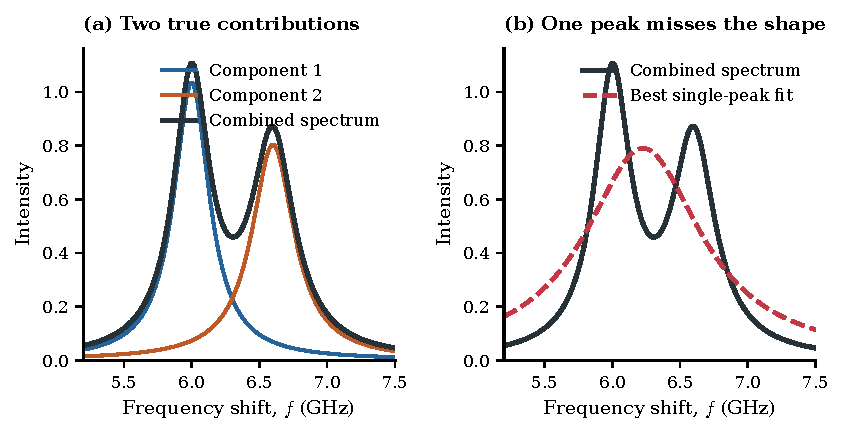
\includegraphics[width=1.0\linewidth]{figures/figure_07_single_peak_limit.pdf}
\caption{A single peak misses the shape of this chosen two-component mixture. (a) The true components and their sum. (b) The same sum and its best single-Lorentzian least-squares fit. The panels have common frequency and intensity scales. Stronger overlap can make the mismatch less apparent.}
\label{fig:single_peak_fit}\end{figure}

\subsubsection{Methods for known and unknown spectra}

Known component spectra allow their coefficients to be estimated using nonnegative least squares (NNLS). When the spectra are unknown, methods must infer them from variation across the dataset. Principal component analysis (PCA) identifies directions of variation around the mean spectrum; the principal-component loading is not itself a material spectrum. Extreme reconstructed observations in a PCA subspace can instead provide candidate endmembers \citep{mahmodi2024}. This strategy can fail to identify pure materials when all observations remain mixtures.

Vertex component analysis (VCA) searches for endmembers using the geometry of a spectral dataset and relies on the presence of pure observations under its standard formulation \citep{nascimento2005}. Multivariate curve resolution--alternating least squares (MCR-ALS) estimates nonnegative component spectra and coefficients together, but constraints do not necessarily eliminate ambiguity \citep{dejuan2014}. Figure~\ref{fig:known_unknown_unmixing} contrasts the known- and unknown-spectrum problems. Their different assumptions motivate evaluating the recovered components against known simulated truth as well as measuring spectral reconstruction error.

\begin{figure}[htbp]\centering
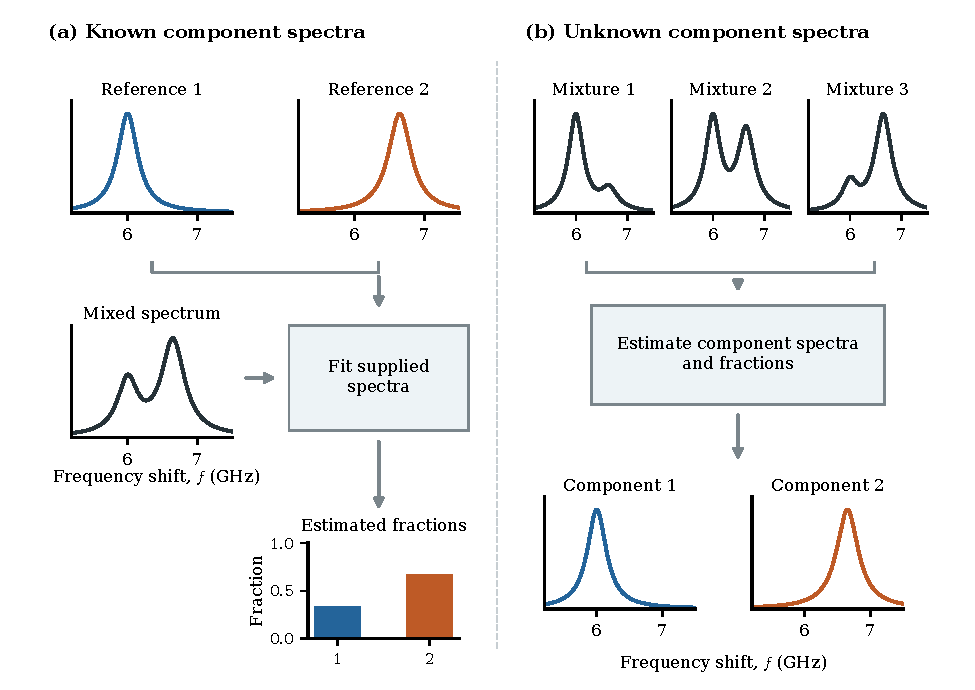
\includegraphics[width=1.0\linewidth]{figures/figure_08_unmixing_workflow.pdf}
\caption{Known and unknown spectral unmixing. Known references permit fitting of contributions; unknown references must be estimated from variation across mixed measurements. Each small spectrum is one continuous curve in the Brillouin band. Recovered outputs are illustrative, not benchmark results.}
\label{fig:known_unknown_unmixing}\end{figure}

\subsubsection{Responses that vary with concentration}

A continuously varying composition requires a family of local responses rather than two fixed endmembers. Water--glycerol solutions provide a useful model system because published Brillouin measurements show composition-dependent shifts and linewidths \citep{adichtchev2019}. If the response at every concentration is supplied, the inverse problem is to estimate the distribution of contributing concentrations. If that response family is unknown, both the spectral relationship and the contributions become uncertain. Even a correct reconstruction cannot by itself assign an absolute concentration to every recovered spectrum. This study will therefore distinguish recovery of concentration distributions with a known calibration from recovery in BFS coordinates without that calibration.

\subsection{Research question and scope}
\label{sec:aims}

This study asks how spectral overlap, photon counts and prior knowledge affect recovery of component responses and their contributions in simulated Brillouin scans. The comparison will use water--glycerol models with an initial range of 0--10\% glycerol by mass. This range is a starting condition: if pilot simulations provide insufficient contrast for a useful comparison, or make recovery too easy to distinguish the methods, it may be revised. Any revision will be documented before final evaluation and applied consistently across the relevant comparisons.

Four configurations separate two questions: whether the sample contains fixed or varying spectral responses, and whether those responses are supplied to the analysis. The configurations are (1) fixed components with known spectra, (2) fixed components with unknown spectra, (3) varying concentrations with a known response family and (4) varying concentrations with an unknown response family. Figure~\ref{fig:study-design} summarises the design. Their objectives are to estimate contributions, recover spectral responses where identifiable, compare performance as conditions change and distinguish spectral reconstruction from recovery of the quantities used to generate the data.

\begin{figure}[htbp]\centering
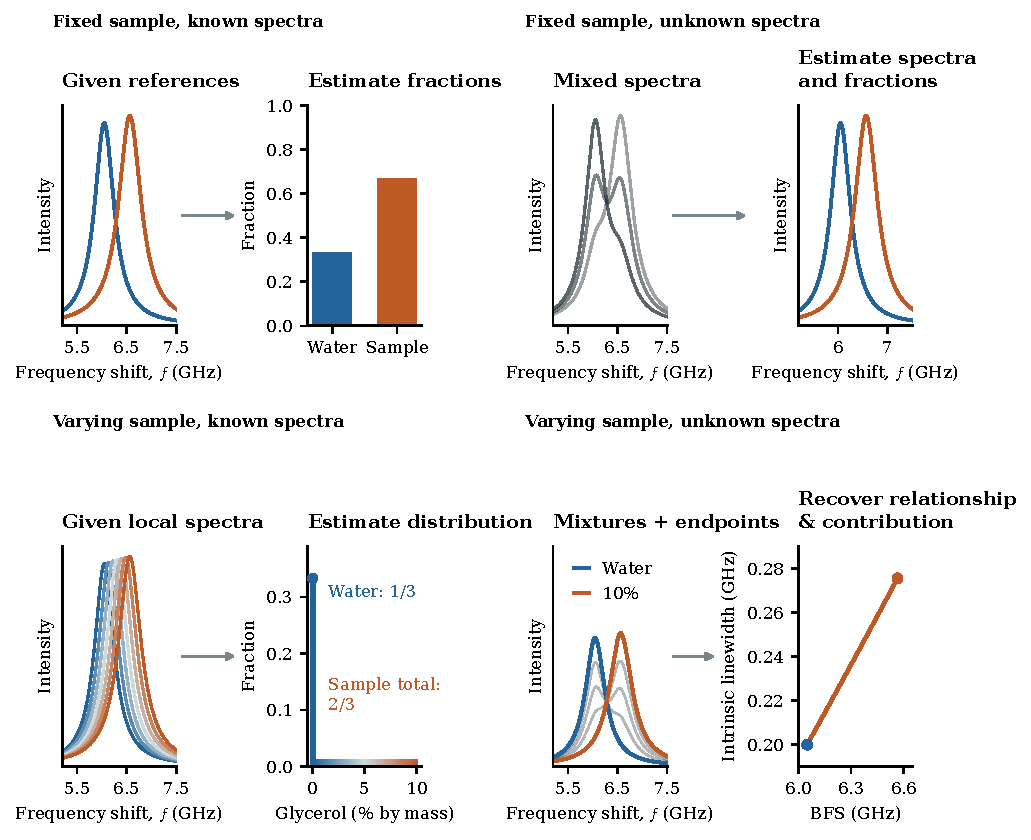
\includegraphics[width=1.0\linewidth]{figures/figure_09_study_questions.pdf}
\caption{Four simulation configurations and their recovery targets. (1) Known fixed spectra are used to estimate mixture weights. (2) Unknown fixed spectra require estimation of component spectra and weights. (3) Known concentration-dependent spectra are used to estimate a concentration distribution. (4) Unknown varying spectra require estimation of contributions and spectral relationships. The final panel illustrates the prescribed BFS (blue dashed line, left axis) and intrinsic linewidth (orange solid line, right axis) versus glycerol mass percentage. All example outputs are schematic, not recovery results. Unknown-spectrum weights require intensity calibration to represent collection fractions; the final configuration does not imply uniquely recoverable absolute concentration.}
\label{fig:study-design}\end{figure}

The study is limited to spectral analysis of simulated two-dimensional scans generated from three-dimensional concentration fields. Geometry will provide ground truth for the mixtures, but the positions of the contributing signals along the collection axis will not be reconstructed. Experimental validation and conversion of recovered spectra into mechanical moduli are outside scope. The unknown-spectrum configuration will be treated as an investigation of recoverability, not as a guarantee that an arbitrary response family has a unique solution.

\clearpage
\section{Methodology}
\subsection{Simulation design and baseline conditions}

Two datasets will be generated from the same prescribed geometry: a homogeneous glycerol-containing region in water and a region whose concentration varies continuously. Each will be analysed with known and unknown responses, giving the four configurations in Section~\ref{sec:aims}. Conditions will be varied in controlled comparisons, and all methods within a comparison will receive the same simulated observations. The initial baseline in Table~\ref{tab:conditions} defines a reproducible example, including the figures in this draft; these are proposed computational conditions rather than measured experimental settings.

\begin{table}[htbp]\centering\small
\caption{Proposed baseline simulation conditions. Sensitivity settings are specified in the text.}
\label{tab:conditions}
\begin{tabular}{@{}p{0.40\linewidth}p{0.53\linewidth}@{}}\toprule
Quantity & Baseline value \\ \midrule
Glycerol mass fraction & $0\leq\wg\leq0.10$ \\
Temperature and vacuum wavelength & 296 K and 660 nm \\
Scattering geometry & Ideal backscattering, $\theta=180^\circ$ \\
Sample and scan & Sphere of radius $r_s=20\,\mu\mathrm m$; $x,y=-25,\ldots,25\,\mu\mathrm m$ at $1\,\mu\mathrm m$ spacing \\
Axial collection & Uniform over $0\leq z\leq30\,\mu\mathrm m$; unit integral \\
Depth quadrature & 120 midpoint samples at $0.25\,\mu\mathrm m$ spacing \\
Frequency bins & 401 centres from 4.50 to 8.50 GHz; width 0.01 GHz \\
Local water response & $f_{\mathrm B0}=6.05$ GHz, $\Gamma_0=0.20$ GHz, $A_0=1$ arbitrary area unit \\
Composition coefficients & $a=0.85$, $b=2.0$, $\delta_A=+0.20$ \\
Instrument model & Unit-area Lorentzian; $\Gamma_h=0.276$ GHz \\
Concentration exponent & $\beta=1$ for baseline illustrations \\
Noise and background & Shot noise only; $b_i=0$ initially; noiseless reference retained \\
Photon budgets & $P=10^2,10^3,10^4,10^5$ expected water-reference photons per retained band \\
Noise repetitions & 30 independent realisations per condition \\
\bottomrule\end{tabular}\normalsize
\end{table}

The 660 nm wavelength and elongated collection geometry are motivated by the reference microscope described by \citet{mahmodi2024}, which used a six-pass tandem scanning Fabry--Perot interferometer. That work reports approximate collection dimensions of $2\times2\times100\,\mu\mathrm m$ for the $20\times$ objective and $0.5\times0.5\times10\,\mu\mathrm m$ for the $60\times$ objective, and a spectral resolution of approximately 276 MHz. Here the illustrative baseline collection length is 30 $\mu\mathrm m$, while a Lorentzian instrument response of FWHM 276 MHz is an assumed approximation. The axial top-hat weighting, numerical sampling and sphere size are simulation choices; they are not a measured point-spread function. The numerical frequency step of 10 MHz is not an assertion of 10 MHz instrument resolution.

\subsection{Sample composition and local spectral response}

Glycerol concentration will be expressed as mass fraction,
\begin{equation}
 \wg=\frac{m_{\mathrm g}}{m_{\mathrm g}+m_{\mathrm w}},\qquad 100\wg=\text{glycerol percentage by mass},
 \label{eq:glycerol_fraction}
\end{equation}
where $m_{\mathrm g}$ and $m_{\mathrm w}$ denote glycerol and water masses. The subscript $\mathrm g$ identifies glycerol. For a spherical region centred at the origin, let $d(\mathbf r)=\|\mathbf r\|/r_s$. The two prescribed concentration fields are
\begin{align}
 w_{\mathrm{fixed}}(\mathbf r)&=
 \begin{cases}\wmax,&d<1,\\0,&d\geq1,\end{cases} \\
 w_{\mathrm{varying}}(\mathbf r)&=
 \begin{cases}\wmax(1-d)^\beta,&d<1,\\0,&d\geq1,\end{cases}
 \qquad \beta>0.
 \label{eq:concentration_profile}
\end{align}
Figure~\ref{fig:sample_models_3d} shows both prescribed fields in three dimensions and identifies the collection range.

\begin{figure}[htbp]\centering
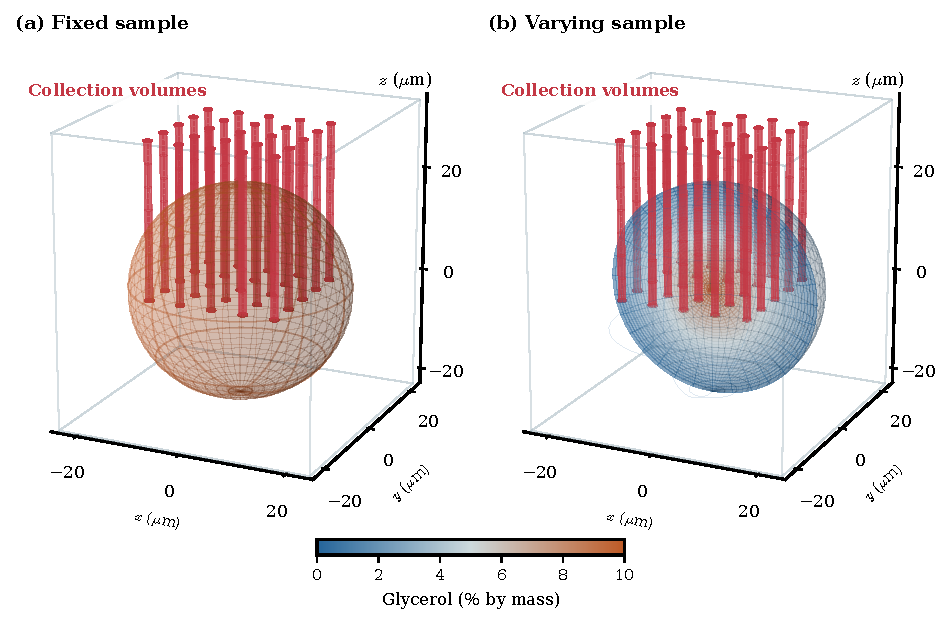
\includegraphics[width=1.0\linewidth]{figures/figure_10_sample_models_3d.pdf}
\caption{Three-dimensional sample definitions. A uniform 10\% solution and a radial gradient are surrounded by water. The gradient cutaway reveals prescribed internal concentration. The red array shows collection regions at representative lateral scan positions, each spanning the 30 $\mu\mathrm m$ axial collection range, from the sample centre at $z=0$ to $z=30\,\mu\mathrm m$. These are simulation test objects, not reconstructed volumes or diffusion predictions.}
\label{fig:sample_models_3d}\end{figure}

These fields define mathematical test objects, not equilibrium droplets or physical diffusion models. Water and a homogeneous 10\% glycerol solution are the two spectral components in the fixed case; the dissolved glycerol and water inside that homogeneous solution are not assigned separate pure-material peaks. In the varying case, a continuum of homogeneous local solution responses contributes to each spectrum. Profiles with $\beta=0.5,1,2$ will test different rates of spatial variation.

The local positive-shift Brillouin band will be represented by a Lorentzian,
\begin{equation}
 R(f;\wg)=\frac{A(\wg)}{\pi}
 \frac{\Gamma(\wg)/2}{[f-f_{\mathrm B}(\wg)]^2+[\Gamma(\wg)/2]^2},
 \qquad \int_{-\infty}^{\infty}R(f;\wg)\,df=A(\wg).
 \label{eq:component_spectrum}
\end{equation}
Its parameters are BFS, intrinsic FWHM and integrated intensity. Integrated intensity is the peak area, not the peak height: the height is $2A/(\pi\Gamma)$ and falls as linewidth increases when area is held fixed. The retained finite frequency band captures only part of the Lorentzian area, which will be accounted for in the count calculation. Neither the Rayleigh peak nor the negative-shift Brillouin band is included in this simulation.

The baseline composition dependence is prescribed as
\begin{align}
 f_{\mathrm B}(\wg)&=f_{\mathrm B0}(1+a\wg), \label{eq:bfs_model}\\
 \Gamma(\wg)&=\Gamma_0\left[\left(\frac{f_{\mathrm B}(\wg)}{f_{\mathrm B0}}\right)^2+b\wg\right], \label{eq:linewidth_model}\\
 A(\wg)&=A_0\left(1+\delta_A\frac{\wg}{\wmax}\right). \label{eq:intensity_model}
\end{align}
Published solution measurements motivate a concentration-dependent response \citep{adichtchev2019}, but the coefficients in Table~\ref{tab:conditions} are provisional model choices retained from the working draft. They are not a fit to that paper's data at 660 nm and 296 K. In particular, Equation~\ref{eq:linewidth_model} is a phenomenological simulation law, not a universal relation between glycerol concentration and damping. At 10\% by mass the prescribed BFS is 6.56425 GHz and intrinsic linewidth is approximately 0.27545 GHz, compared with 6.05 GHz and 0.20 GHz for water.

Integrated intensity will increase linearly in the baseline, with $\delta_A=+0.20$, so that the 10\% solution has 1.20 times the full-band area of water. This is a prescribed simulation choice because no verified intensity calibration has been supplied. Constant-area ($\delta_A=0$) and decreasing-area ($\delta_A=-0.20$) cases can test sensitivity to this assumption; none is presented as a measured trend. Figure~\ref{fig:concentration_parameters} shows all three prescribed quantities. Wider concentration ranges, if adopted after pilot evaluation, will require reconsidering the response laws rather than assuming that these approximations remain valid indefinitely.

\begin{figure}[htbp]\centering
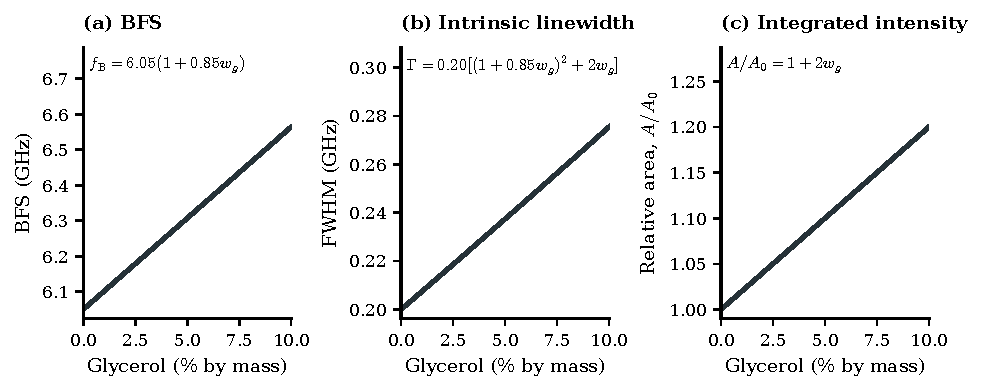
\includegraphics[width=1.0\linewidth]{figures/figure_13_concentration_parameters.pdf}
\caption{Here $w$ denotes glycerol mass fraction (percentage divided by 100). Prescribed response laws over the initial 0--10\% glycerol mass range. BFS and intrinsic linewidth follow the provisional model. Integrated intensity is chosen to increase linearly by 20\% across this range. The curves are simulation inputs, not measured or fitted calibrations; integrated intensity means peak area.}
\label{fig:concentration_parameters}\end{figure}

\subsection{Collection model and noiseless dataset}
\label{sec:geometry}

Each scan position will collect a weighted combination of responses along the optical axis. Neglecting lateral averaging in the baseline, the ideal spectrum is
\begin{equation}
 s_i(f)=\int_{0}^{L_z}W_i(z)R(f;w_i(z))\,dz,
 \qquad W_i(z)\geq0,\qquad \int W_i(z)\,dz=1.
 \label{eq:depth_integrated_spectrum}
\end{equation}
Here $w_i(z)$ is the local mass fraction at $(x_i,y_i,z)$. The baseline uses $W_i=1/L_z$ within the collection interval $0\leq z\leq L_z$ and zero outside it. This interval starts at the sample midplane and traverses one side of the sphere. Normalising the weighting keeps the reference signal comparable as collection length is varied; it isolates mixture composition from a separate change in collected brightness. A physical count rate would additionally depend on collection efficiency and illumination. These factors are represented separately by the count scale below.

For the fixed sample, Equation~\ref{eq:depth_integrated_spectrum} reduces exactly to
\begin{equation}
 s_i(f)=(1-p_i)R(f;0)+p_iR(f;\wmax),\qquad
 p_i=\int W_i(z)\,\mathbf{1}_{\{d(x_i,y_i,z)<1\}}\,dz.
 \label{eq:fixed_mixture}
\end{equation}
The coefficient $p_i$ is a collection-weighted fraction of the homogeneous sample region, not its glycerol mass fraction. With constant $A$, it is also the full-band sample signal fraction. With concentration-dependent $A$, the signal fraction becomes
\begin{equation}
 p_i^{\mathrm{signal}}=
 \frac{p_i A(\wmax)}{(1-p_i)A(0)+p_i A(\wmax)}.
 \label{eq:signal_fraction}
\end{equation}
For $r_s=20\,\mu\mathrm m$ and $L_z=30\,\mu\mathrm m$, the central ray has $p_i=2/3$. No ray contains a pure sample response in this baseline. This provides a deliberate test of methods that depend on observing pure endmembers. A separate 10 $\mu\mathrm m$ collection-length condition will permit pure sample rays in the fixed case.

Figure~\ref{fig:fixed_formation} follows the central collection ray from the three-dimensional model to its two weighted spectral contributions and their sum.

\begin{figure}[htbp]\centering
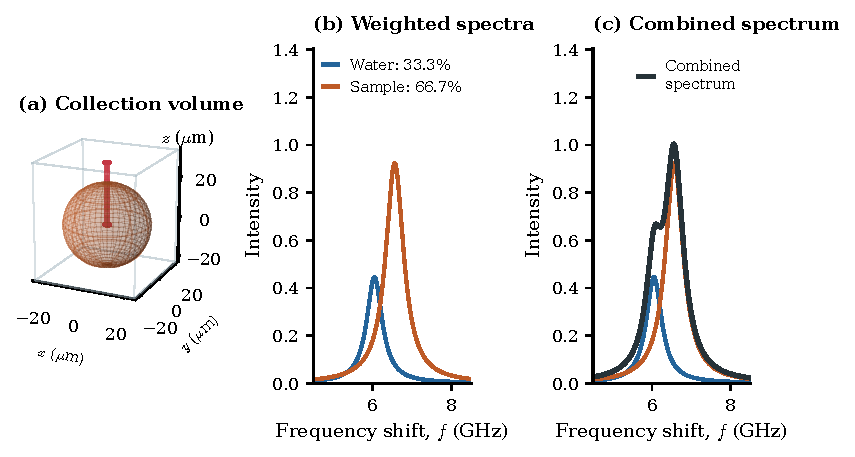
\includegraphics[width=1.0\linewidth]{figures/figure_11_fixed_mixture_3d.pdf}
\caption{Formation of a fixed-component spectrum along one collection ray. The central ray contains collection fractions 33.3\% water and 66.7\% homogeneous 10\% solution (full-band signal fractions 29.4\% and 70.6\%, respectively). Coloured curves include these weights and the concentration-dependent response areas; their exact sum is black. The spectra include the assumed instrument response. Intensity denotes spectral density in the common arbitrary scale.}
\label{fig:fixed_formation}\end{figure}

For the varying sample, it is useful to describe the collection-weighted distribution of concentrations by a probability measure $\nu_i$. Then
\begin{equation}
 s_i(f)=\int_{[0,\wmax]}R(f;w)\,d\nu_i(w),\qquad
 \nu_i(B)=\int W_i(z)\,\mathbf{1}_{\{w_i(z)\in B\}}\,dz.
 \label{eq:continuous_unmixing}
\end{equation}
The measure notation includes discrete contributions such as surrounding pure water as well as continuous concentration distributions. A smooth probability density alone would omit the point mass at zero concentration. In numerical fitting, $\nu_i$ will be represented by nonnegative probability masses on concentration bins, and ground truth will be obtained using the same collection weights as the forward simulation.

Figure~\ref{fig:varying_formation} expands the corresponding process for the varying sample, showing local responses at immediate depth positions within one collection volume. These depths are distinct from the lateral scan positions in Figure~\ref{fig:noiseless_dataset}.

\begin{figure}[htbp]\centering
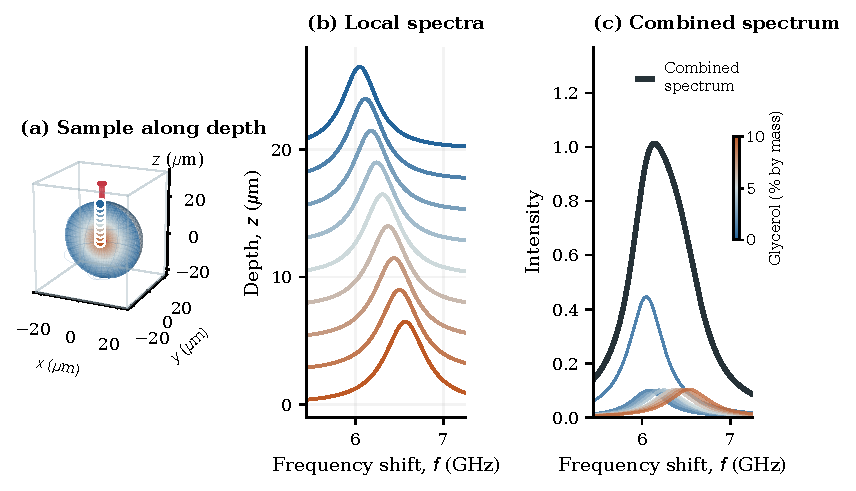
\includegraphics[width=1.0\linewidth]{figures/figure_12_varying_mixture_depth.pdf}
\caption{Formation of a varying-concentration spectrum. (a) Coloured points lie at different depths within one collection region. (b) Local spectra are individually scaled and offset vertically for visibility. (c) Water and concentration-bin contributions are depth-weighted and summed exactly. The colour bar identifies glycerol concentration for the coloured contributions. Colour represents glycerol mass fraction. Collection begins at the centre and traverses one side of the gradient. These are depth contributions to one pixel, not different lateral pixels.}
\label{fig:varying_formation}\end{figure}

The noiseless recorded spectrum includes instrument broadening:
\begin{align}
 y_i^{(0)}(f)&=(h*s_i)(f)+b_i(f), \label{eq:noiseless_recorded}\\
 (h*s_i)(f)&=\int_{-\infty}^{\infty}h(f-f')s_i(f')\,df',\qquad
 \int h(f)\,df=1. \label{eq:convolution}
\end{align}
The asterisk denotes convolution, not multiplication. The baseline $h$ is a Lorentzian with FWHM $\Gamma_h=0.276$ GHz and $b_i=0$. Convolution of two Lorentzians preserves area and adds their FWHMs, allowing this particular forward model to be calculated analytically before depth integration. A narrow-response sensitivity case with $\Gamma_h=0.10$ GHz will help distinguish effects of instrument broadening from mixture overlap. Fits will use the same stated instrument response, so the recovered local linewidth refers to the intrinsic response. Noiseless means that random count fluctuations have not been drawn; it does not mean that instrumental broadening has been removed.

\begin{figure}[htbp]\centering
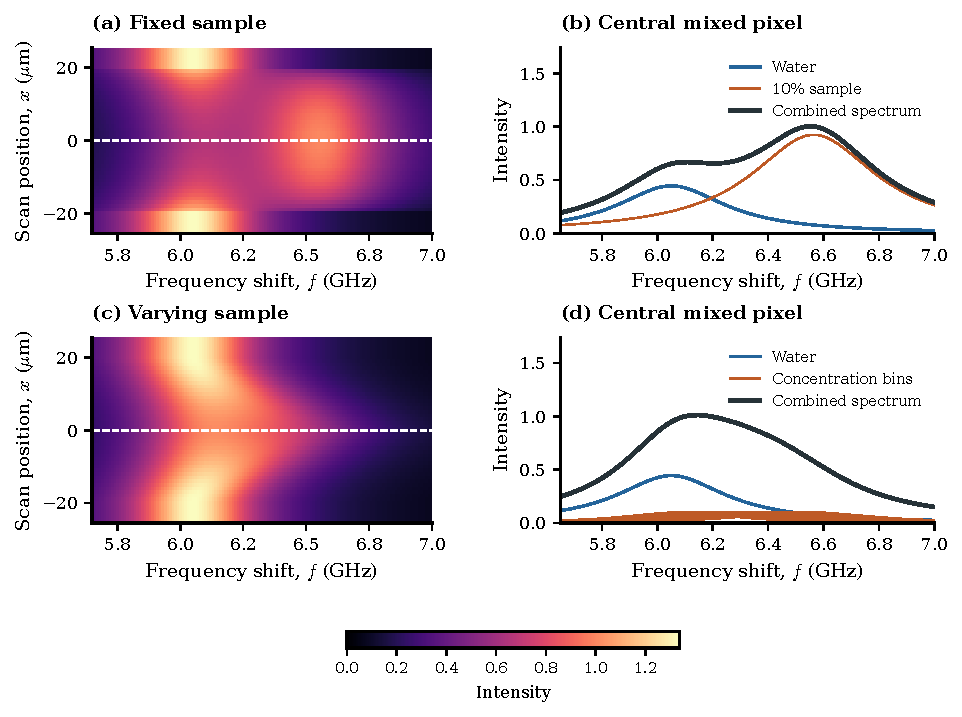
\includegraphics[width=1.0\linewidth]{figures/figure_14_noiseless_dataset.pdf}
\caption{Noiseless forward-model datasets. Left: three-dimensional sample models and red collection indicators. Middle: the central lateral spectral line, displayed over 5.65--7.00 GHz; the complete simulated band is 4.50--8.50 GHz. The white line selects $x=y=0$. Right: contributions to that single pixel and their exact black sum. Intensity denotes spectral density on the common arbitrary scale. Both rows use common scales. Instrument broadening and the chosen increasing-intensity law are included; random noise and additive background are absent.}
\label{fig:noiseless_dataset}\end{figure}

Figure~\ref{fig:noisy_dataset} shows matching Poisson-noise examples at a reference budget of 10000 water photons per pixel.

\begin{figure}[htbp]\centering
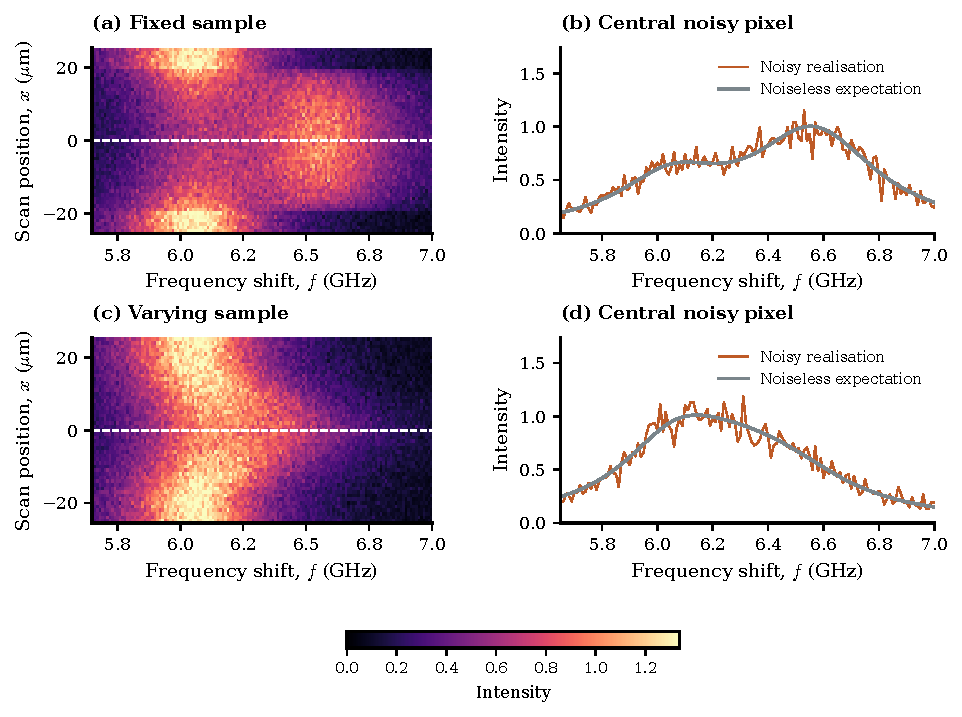
\includegraphics[width=1.0\linewidth]{figures/figure_15_noisy_dataset.pdf}
\caption{Poisson-noise examples corresponding to Figure~\ref{fig:noiseless_dataset}, with the same geometry and heatmap colour limits. The reference budget is 10000 expected water photons per pixel in the full band. Counts are converted to spectral density (labelled intensity) using the known count scale and bin width for display. Orange traces show noisy pixels and faint curves show their expectations. These are simulations, not experimental measurements.}
\label{fig:noisy_dataset}\end{figure}

Figure~\ref{fig:noiseless_dataset} shows the form of the data that the analysis will receive. A two-dimensional spatial scan produces a cube indexed by $x$, $y$ and frequency, or equivalently a matrix with one spectrum per spatial position. The displayed line-scan window is narrowed to 5.65--7.00 GHz to make the spectral variation visible, without changing the simulated frequency bins. The right-hand panels decompose the central mixed pixel into contributions whose sum equals the corresponding line-scan spectrum. The observed spectra mix sample and water because the collection interval extends beyond the sample. The central fixed-sample ray now has two-thirds sample weighting and one-third water weighting. The fixed and varying samples can therefore both display smoothly changing measured spectra even though their local composition fields are different. Recovery will be tested against the known contribution distributions, rather than by interpreting the apparent peak position as a direct concentration map.

\subsection{Photon statistics and simulation comparisons}

Photon shot noise will be generated by sampling independent Poisson counts conditional on the expected spectrum:
\begin{equation}
 N_{im}\sim\operatorname{Poisson}(\mu_{im}),\qquad
 \mu_{im}=t_i\kappa\int_{\Delta f_m}y_i^{(0)}(f)\,df.
 \label{eq:noise_model}
\end{equation}
The scale $\kappa$ converts the arbitrary spectral area into photon rate, and $t_i$ is acquisition time. The same bin integration will be applied to model spectra and data. If an additive background is introduced, it will be included in $y_i^{(0)}$ before sampling, so its photons also contribute shot noise. Detector read noise and drift will be excluded from the primary benchmark and reported as exclusions; a separate extension would need independently specified distributions or drift trajectories.

Noise conditions will be set by expected photon budget rather than by assigning an uncalibrated acquisition time. Let $J_0$ be the integral of the instrument-broadened water response over the retained frequency bins. For each budget $P$, choose $t_i\kappa=P/J_0$. Pure water then has $P$ expected photons in the retained band, while mixtures retain any change in finite-band area or modelled intensity. This scaling is held constant across scan positions in a comparison. The proposed budgets are $10^2$, $10^3$, $10^4$ and $10^5$, with 30 independent noise realisations at each budget and a separate noiseless condition. Counts will not be converted to seconds without a measured photon rate. The exposure-time illustration in Figure~\ref{fig:noise} separately assumes 1000 expected water-reference photons per second within its displayed 5.25--7.35 GHz band. That assumed rate defines the illustrative seconds and is not a calibration of the reference microscope; the main benchmark remains specified by photon budgets.

Pilot development will use the baseline sample and the planned variations $\beta=0.5,1,2$, $L_z=10,30,100\,\mu\mathrm m$, $\Gamma_h=0.10,0.276$ GHz and $\delta_A=-0.20,0,+0.20$. Initially, each factor will be varied separately from the baseline to make its effect interpretable. Additional overlap tests will vary the maximum concentration to 2.5\%, 5\% and 10\% within the initial range. A separate evaluation set with radii 15 and 25 $\mu\mathrm m$ and exponents 0.75 and 1.5 will be reserved before tuning. Lateral step and depth step will each be halved in a numerical convergence check; a metric change greater than 1\% will trigger refinement. These choices define a proposed benchmark and can be revised during pilot work before the final protocol is frozen.

\subsection{Analysis of the four configurations}
\subsubsection{Fixed components with known spectra}

NNLS will estimate component coefficients from the known water and homogeneous-solution responses. The dictionary $\mathbf D$ will contain the instrument-broadened, bin-integrated reference responses with their prescribed areas retained. On count-rate-equivalent data, the fit is
\begin{equation}
 \widehat{\mathbf a}_i=\underset{\mathbf a_i\geq0}{\operatorname{argmin}}
 \|\mathbf y_i-\mathbf D\mathbf a_i\|_2^2,
 \qquad \widehat p_{ik}=\frac{\widehat a_{ik}}{\sum_\ell\widehat a_{i\ell}}.
 \label{eq:known_fit}
\end{equation}
Here $\mathbf y_i$ denotes counts divided by the known count scale, and noiseless inputs use the corresponding expected values. A zero coefficient sum will be recorded as failure rather than normalised. Keeping $A$ in the references allows the coefficients to be compared with the collection-weighted ground truth; unit-area references instead produce signal fractions and require the conversion in Equation~\ref{eq:signal_fraction}. NNLS is the primary baseline; its unweighted loss does not exactly match low-count Poisson likelihood, which will be noted when interpreting performance.

\subsubsection{Fixed components with unknown spectra}

PCA-assisted endmember estimation, VCA and MCR-ALS will be compared with the number of material components fixed at two. PCA will first reconstruct spectra from a low-dimensional subspace; extreme observations in that subspace will supply candidate responses. VCA will select candidate endmembers using its standard geometric procedure. Candidate responses will then be fitted across the dataset using NNLS. MCR-ALS will minimise
\begin{equation}
 \min_{\mathbf C\geq0,\,\mathbf S\geq0}
 \|\mathbf Y-\mathbf C\mathbf S^{\mathsf T}\|_{\mathrm F}^{2},
 \label{eq:mcr}
\end{equation}
where rows of $\mathbf Y$ are spectra, columns of $\mathbf S$ are component responses and rows of $\mathbf C$ contain their coefficients. Multiple initialisations will assess sensitivity to local solutions. Spectrum scaling will be fixed by a stated area convention, and components will be matched to truth by testing both label assignments. These steps remove scale and label conventions but do not resolve all mixture ambiguity.

The 30 $\mu\mathrm m$ baseline intentionally contains pure-water rays but no pure-sample ray. Extreme observations can therefore remain mixtures, even without noise, and this will be reported as an assumption limitation rather than attributed entirely to optimisation failure. A reference-assisted comparison will fix the water spectrum using the mean of designated water-only calibration positions. Their known location is additional supplied information and will be declared as such. An unassisted comparison will not receive those labels. In the intensity-sensitivity cases, physical collection fractions will not be claimed for unknown-area components without an area calibration; normalised signal fractions will be evaluated instead.

\subsubsection{Varying concentrations with known spectra}

A concentration dictionary will represent the known local response family, including its instrument response and bin integration. The initial grid will contain 51 concentration values from 0 to $\wmax$; coefficients will be probability masses rather than density values. For $\wmax=0.10$, the spacing is 0.002 in mass fraction, or 0.2 percentage points. With a nonnegative coefficient vector $\mathbf u_i$, fitting will use
\begin{equation}
 \widehat{\mathbf u}_i=\underset{\mathbf u_i\geq0}{\operatorname{argmin}}
 \left[\|\mathbf y_i-\mathbf D\mathbf u_i\|_2^2+
 \eta\|\mathbf L\mathbf u_{i,+}\|_2^2\right],\qquad
 \widehat\pi_{ij}=\frac{\widehat u_{ij}}{\sum_\ell\widehat u_{i\ell}}.
 \label{eq:regularised_distribution}
\end{equation}
The vector $\mathbf u_{i,+}$ contains only positive-concentration bins, preserving a separate unpenalised water atom at zero. The second-difference matrix $\mathbf L$ penalises roughness across the equally spaced positive bins. Dictionaries will be scaled consistently during tuning, and $\eta$ will be selected on development simulations from $0,10^{-6},10^{-5},\ldots,10^2$, then frozen for final evaluation. Halving the concentration-grid spacing will test discretisation sensitivity. Ground-truth bin masses will use a documented nearest-grid assignment, and the same assignment will be retained when comparing cumulative distributions.

Broadening makes neighbouring dictionary columns similar, so a successful spectrum fit may not recover a narrow concentration distribution accurately. The analysis will therefore report the resolution of recovered distributions and their dependence on regularisation. The known response areas permit evaluation of collection-weighted concentration distributions; this interpretation relies on the supplied intensity model and will be reassessed in the intensity-sensitivity cases.

\subsubsection{Varying concentrations with unknown spectra}

Without a concentration calibration, the analysis will be formulated in BFS coordinates. Linewidth and integrated response will be represented by shared smooth functions,
\begin{equation}
 \Gamma=G(f_{\mathrm B}),\qquad A=H(f_{\mathrm B}),\qquad
 s_i(f)=\int \ell(f;u,G(u))\,d\xi_i(u),
 \label{eq:unknown_family}
\end{equation}
where $\ell$ is a unit-area Lorentzian and $\xi_i$ is a nonnegative spectral-area measure over BFS $u$. Its normalised form describes signal contributions. This parameterisation avoids claiming that the data separately determine local intensity and material amount: multiplying an unknown local response area by a function and dividing its contribution weights by the same function can preserve the spectrum. The linewidth function can also trade off against the spread of centres, so a unique solution will not be assumed.

The initial implementation will jointly fit nonnegative BFS-bin weights and a positive linewidth function. The linewidth function will be represented by a piecewise-linear curve with five equally spaced knots over the fitted BFS interval; a second-difference penalty on the knot values will control roughness. Alternating constrained updates will start from ten initialisations, with regularisation selected using development data. Water-only and water-plus-10\%-solution reference conditions will fix the corresponding endpoint responses. The primary distribution estimates will be signal-weighted, because the baseline response area varies with concentration. A reference-assisted branch may supply $H$ from the simulation model to investigate the value of intensity calibration; a constant-$H$ branch will be a deliberate model-mismatch comparison rather than an assumption that the baseline has constant area. Recovering an arbitrary unknown $H$ and a physical concentration distribution simultaneously will not be treated as an identifiable task on the basis of one or two reference spectra alone.

Evaluation will compare the recovered $G$ and signal-weighted BFS distributions with their true counterparts. Under constant area these distributions coincide with collection-weighted distributions; under varying area their ground truth will be intensity-weighted. An absolute concentration axis will be reported only when a concentration-to-BFS calibration is explicitly supplied. This formulation allows the fourth configuration to test how much spectral information is recoverable while keeping its unresolved ambiguities visible.

\subsection{Accuracy and robustness evaluation}

Recovery accuracy will be evaluated separately from spectral reconstruction. For fixed components, the primary contribution error is
\begin{equation}
 \mathrm{MAE}_{p}=\frac{1}{N}\sum_i|\widehat p_i-p_i|.
 \label{eq:proportion_mae}
\end{equation}
The reported fraction will be identified as collection-weighted or signal-weighted according to the response normalisation. Unknown component responses will additionally be compared by absolute BFS error, absolute intrinsic-linewidth error and relative area error when their areas are calibrated. Components will be matched before these errors are calculated, and the denominator convention for any relative error will be reported.

For varying responses, distributions will be compared using the one-dimensional Wasserstein distance,
\begin{equation}
 W_{1,i}=\int|\widehat F_i(x)-F_i(x)|\,dx.
 \label{eq:wasserstein}
\end{equation}
Here $F_i$ and $\widehat F_i$ are cumulative probability distributions including discrete masses. In the known-family configuration, $x$ is glycerol mass fraction; in the unknown-family configuration it is BFS in GHz, using signal-weighted truth where appropriate. Both the dimensional error and an error divided by the corresponding coordinate range will be reported. Distribution errors will also be reported for sample-intersecting rays separately, so numerous pure-water positions do not hide poor recovery within the sample.

Spectral reconstruction will be measured relative to the noiseless instrument-affected bin values:
\begin{equation}
 \mathrm{NRMSE}_i=
 \sqrt{\frac{\sum_m[\widehat y_{im}-y^{(0)}_{im}]^2}
 {\sum_m[y^{(0)}_{im}]^2}}.
 \label{eq:spectral_nrmse}
\end{equation}
Reconstruction and reference values will be expressed in the same units. This error measures agreement with the expected measurement, not agreement with a particular random noise draw. Small NRMSE accompanied by large component or distribution error will be interpreted as successful reconstruction with unsuccessful recovery.

Numerical failures will be distinguished from inaccurate but converged results. A numerical failure means nonfinite output, a zero total fitted contribution, violated constraints beyond a relative tolerance of $10^{-8}$, or failure to satisfy the stopping rule within 1000 outer iterations for alternating methods. The proposed stopping rule is a relative objective change below $10^{-6}$ for five consecutive iterations. As provisional practical criteria, a fixed-mixture recovery will be flagged if its absolute fraction error exceeds 0.05; a distribution recovery will be flagged if its range-normalised Wasserstein error exceeds 0.05. These are study-defined tolerances, not established physical limits. They will be frozen after pilot assessment and supplemented with continuous error distributions so conclusions do not depend on a single threshold.

For each condition, results will report mean and median error, spread across independent noise realisations, numerical failure rate and the fraction exceeding the practical tolerance. The same random datasets will be paired across methods. The noiseless case will first identify limitations caused by overlap, model ambiguity or discretisation; photon-budget comparisons will then quantify the additional effect of shot noise. Regularisation and other tuning choices will be fixed before evaluation on reserved geometries. The figures in this draft illustrate the forward model only and do not present benchmark results.

\subsection{Computational implementation and reproducibility}

Python will be used to generate spectra, fit the recovery models and calculate errors. Each run will save the concentration field, grid coordinates, frequency-bin edges, collection weights, local response parameters, instrument model, photon budget, random seeds and true contribution distributions. Methods within a comparison will use identical saved inputs. Output metadata will record software versions, solver settings, normalisation, initialisation and stopping criteria, together with any revisions to the initial concentration range or proposed conditions.

Before final comparisons, numerical checks will verify that the local Lorentzian has the stated full-band area, the collection weighting integrates to one, and the fixed-component integral agrees with the analytic mixture. Depth, frequency and concentration discretisations will be refined to check convergence of the reported metrics. The unknown-spectrum analysis will additionally record variation across initialisations rather than reporting only the best-looking solution. The resulting conclusions will concern recovery under the stated simulation assumptions; experimental validation remains outside this study.

\clearpage\bibliography{BrillouinMicroscopy}
\end{document}

